
\documentclass[12pt]{article}
\usepackage[utf8]{inputenc}
\usepackage{tabularx}
\usepackage{fancyhdr}
\usepackage{graphicx}
\usepackage{xcolor}
\pagestyle{fancy}
\fancyhf{}
\rhead{}

\usepackage{sectsty}
\sectionfont{\color{blue!60!black}}
\subsectionfont{\color{blue!80!black}}

\usepackage{titlesec}
\titleformat{\section}{\Large\bfseries\color{blue!80!black}}{\thesection}{1em}{}
\titleformat{\subsection}{\large\bfseries\color{blue!50!black}}{\thesubsection}{1em}{}

\usepackage{hyperref}


\usepackage[spanish]{babel}
\usepackage{graphicx}
\usepackage{float}
\usepackage{amsmath}
\usepackage{booktabs}
\usepackage{geometry}
\geometry{margin=2.5cm}
\usepackage{listings}


\title{Simulación de Eventos Discretos: Sistema de Peaje}
\author{Melani Forsythe Matos}
\date{Abril 2025}

\begin{document}

\setlength{\pdfpageheight}{\paperheight}
\setlength{\pdfpagewidth}{\paperwidth}
\clearpage

\maketitle


\section{Introducción}

\subsection*{Breve descripción del proyecto}
Este proyecto tiene como objetivo desarrollar una simulación basada en eventos discretos de un sistema de peaje en el cual los vehículos llegan de manera aleatoria y son atendidos por varias cabinas disponibles. La simulación busca modelar el flujo vehicular y analizar el rendimiento del sistema bajo diferentes configuraciones operativas.

\subsection*{Objetivos y metas}
\begin{itemize}
    \item Evaluar el impacto de los parámetros del sistema (tasa de llegada, tasa de servicio, número de cabinas, duración de simulación) en métricas clave como el tiempo promedio de espera, la cantidad de autos atendidos y la ocupación de las cabinas.
    \item Validar la coherencia del modelo simulado con los principios teóricos de los sistemas de colas.
    \item Generar visualizaciones estadísticas que faciliten la interpretación de los resultados.
    \item Brindar una herramienta sencilla que permita analizar decisiones operativas en sistemas de atención múltiple.
\end{itemize}

\subsection*{Sistema específico simulado y variables de interés}
El sistema simulado es una estación de peaje con varias cabinas de atención. Las llegadas de vehículos siguen una distribución exponencial (Poisson) y el servicio también es exponencial, lo que define un modelo $M/M/c$. Las variables analizadas fueron:

\begin{itemize}
    \item Tiempo promedio de espera de los vehículos.
    \item Total de vehículos atendidos en cada simulación.
    \item Porcentaje promedio de ocupación de las cabinas.
\end{itemize}

\subsection*{Variables que describen el problema}
\begin{itemize}
    \item $\lambda$: tasa de llegada de vehículos.
    \item $\mu$: tasa de servicio de las cabinas.
    \item $c$: número de cabinas (servidores).
    \item $T$: duración total de la simulación.
    \item $W$: tiempo promedio de espera en cola.
    \item $\rho$: nivel de utilización del sistema.
\end{itemize}

\section{Detalles de Implementación}

\subsection*{1. Modelado del sistema}

Para representar el sistema de peaje como una simulación de eventos discretos, se definió una clase \texttt{Evento}, que modela los eventos de llegada y salida de vehículos. Estos eventos se gestionan en una cola de prioridad que garantiza su procesamiento en orden cronológico:

\begin{lstlisting}[language=Python, caption={Definición de la clase Evento}]
class Evento:
    def __init__(self, tiempo, tipo, cabina_id=None):
        self.tiempo = tiempo
        self.tipo = tipo
        self.cabina_id = cabina_id

    def __lt__(self, otro):
        return self.tiempo < otro.tiempo
\end{lstlisting}

\subsection*{2. Lógica de simulación}

La función \texttt{simular\_peaje(...)} implementa la lógica central. Se inicializa el reloj y se procesan eventos hasta alcanzar el tiempo total de simulación. Cada evento actualiza el estado del sistema:

\begin{lstlisting}[language=Python, caption={Estructura principal de la simulación}]
def simular_peaje(tasa_llegada, tasa_servicio, tiempo_total, num_cabinas):
    reloj = 0
    eventos = []
    heapq.heappush(eventos, Evento(random.expovariate(tasa_llegada), 'llegada'))
    cabinas = [None] * num_cabinas
    cola = []
    tiempos_espera = []
    ocupacion_cabinas = [0] * num_cabinas
    tiempo_anterior = 0

    while eventos:
        evento = heapq.heappop(eventos)
        reloj = evento.tiempo
        ...
\end{lstlisting}

\subsection*{3. Múltiples ejecuciones y configuración}

Se probaron múltiples combinaciones de parámetros, como número de cabinas, tasa de llegada, tasa de servicio y tiempo de simulación. El siguiente fragmento muestra cómo se itera sobre estas combinaciones:

\begin{lstlisting}[language=Python, caption={Ejecución de múltiples simulaciones}]
for cabinas in cabinas_list:
    for tiempo_total in tiempos_totales:
        for tasa_llegada in tasas_llegada:
            for tasa_servicio in tasas_servicio:
                for _ in range(num_simulaciones):
                    espera, atendidos, ocupacion = simular_peaje(
                        tasa_llegada, tasa_servicio, tiempo_total, cabinas)
                    ...
\end{lstlisting}

\subsection*{4. Generación de gráficos y análisis}

Los resultados se almacenaron en un \texttt{DataFrame} y se generaron gráficos estadísticos para visualizar el comportamiento del sistema:

\begin{lstlisting}[language=Python, caption={Ejemplo de generación de gráfico}]
plt.figure(figsize=(8, 5))
sns.histplot(df_resultados["Tiempo promedio espera"], kde=True, bins=20)
plt.title("Distribucin del Tiempo Promedio de Espera")
plt.xlabel("Tiempo promedio de espera (s)")
plt.ylabel("Frecuencia")
plt.tight_layout()
plt.savefig("hist_espera.png")
\end{lstlisting}


\section{Resultados y Experimentos}

\subsection*{Hallazgos de la simulación}
\begin{itemize}
    \item Al aumentar el número de cabinas, se reduce el tiempo promedio de espera y también la ocupación individual de cada cabina.
    \item A tasas de llegada altas y pocas cabinas, el sistema entra en congestión, elevando considerablemente los tiempos de espera.
    \item Las distribuciones de espera son asimétricas, lo cual es esperable en sistemas de colas reales.
\end{itemize}

\subsection*{Interpretación de los resultados}
\begin{itemize}
    \item El modelo refleja de forma realista la dinámica de un peaje: mayor capacidad reduce los cuellos de botella.
    \item El equilibrio entre $\lambda$, $\mu$ y $c$ es crucial para evitar sobrecarga del sistema.
    \item La ocupación y el rendimiento del sistema pueden variar significativamente con pequeños cambios en los parámetros.
\end{itemize}

\subsection*{Hipótesis extraídas de los resultados}
\begin{itemize}
    \item \textbf{H1}: Un mayor número de cabinas reduce significativamente el tiempo de espera.
    \item \textbf{H2}: A igualdad de cabinas, un mayor tiempo total de simulación estabiliza los resultados.
    \item \textbf{H3}: La ocupación promedio es inversamente proporcional al número de cabinas disponibles.
\end{itemize}

\subsection*{Experimentos realizados para validar las hipótesis}
\begin{itemize}
    \item Se probaron combinaciones con 2, 3 y 4 cabinas.
    \item Se variaron tasas de llegada (1/4 y 1/5) y servicio (1/3 y 1/4).
    \item Cada configuración fue simulada 10 veces para asegurar consistencia estadística.
\end{itemize}

\subsection*{Necesidad de realizar análisis estadístico}
Dado que los eventos de llegada y servicio son aleatorios, cada simulación produce resultados diferentes. Por lo tanto:
\begin{itemize}
    \item Se realizó un análisis estadístico sobre los resultados con medias, desviaciones estándar, mínimos y máximos.
    \item Se graficaron las distribuciones para facilitar la visualización del comportamiento agregado.
\end{itemize}

\subsection*{Análisis de parada de la simulación}
Para garantizar resultados estables, se utilizaron tiempos de simulación de 300 y 500 unidades. Se observó que:
\begin{itemize}
    \item Con duraciones menores, las colas aún no alcanzaban estado estacionario.
    \item Para tiempos mayores o iguales a 500, los indicadores clave mostraban menor variabilidad, sugiriendo una buena elección del horizonte de simulación.
\end{itemize}
\newpage

\section{Resultados y Experimentos}
\subsection*{Gráficos}
\begin{figure}[H]
\centering\vspace{-0.5em}
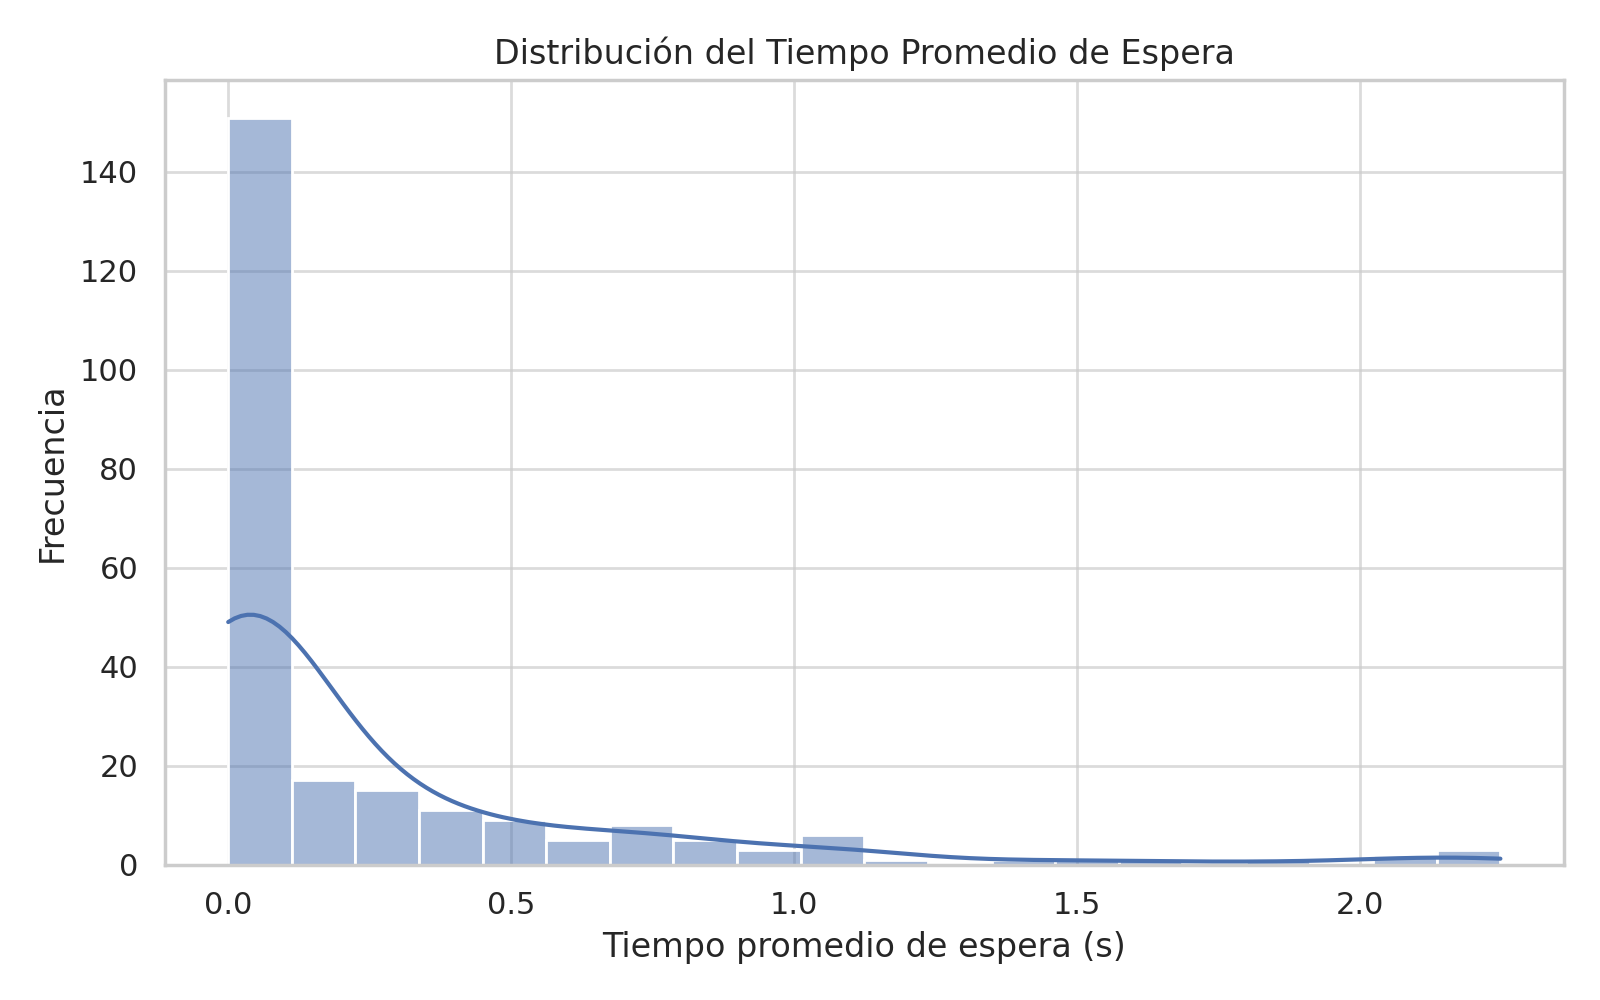
\includegraphics[width=0.8\textwidth]{hist_espera.png}
\caption{Distribución del tiempo promedio de espera en distintas configuraciones.}
\small La mayoría de las simulaciones muestran tiempos de espera inferiores a 1 segundo, indicando eficiencia del sistema. Sin embargo, se observa una cola hacia la derecha, reflejando que ciertas configuraciones (por ejemplo, con pocas cabinas) pueden generar demoras mayores.

\end{figure}

\begin{figure}[H]
\centering\vspace{-0.5em}
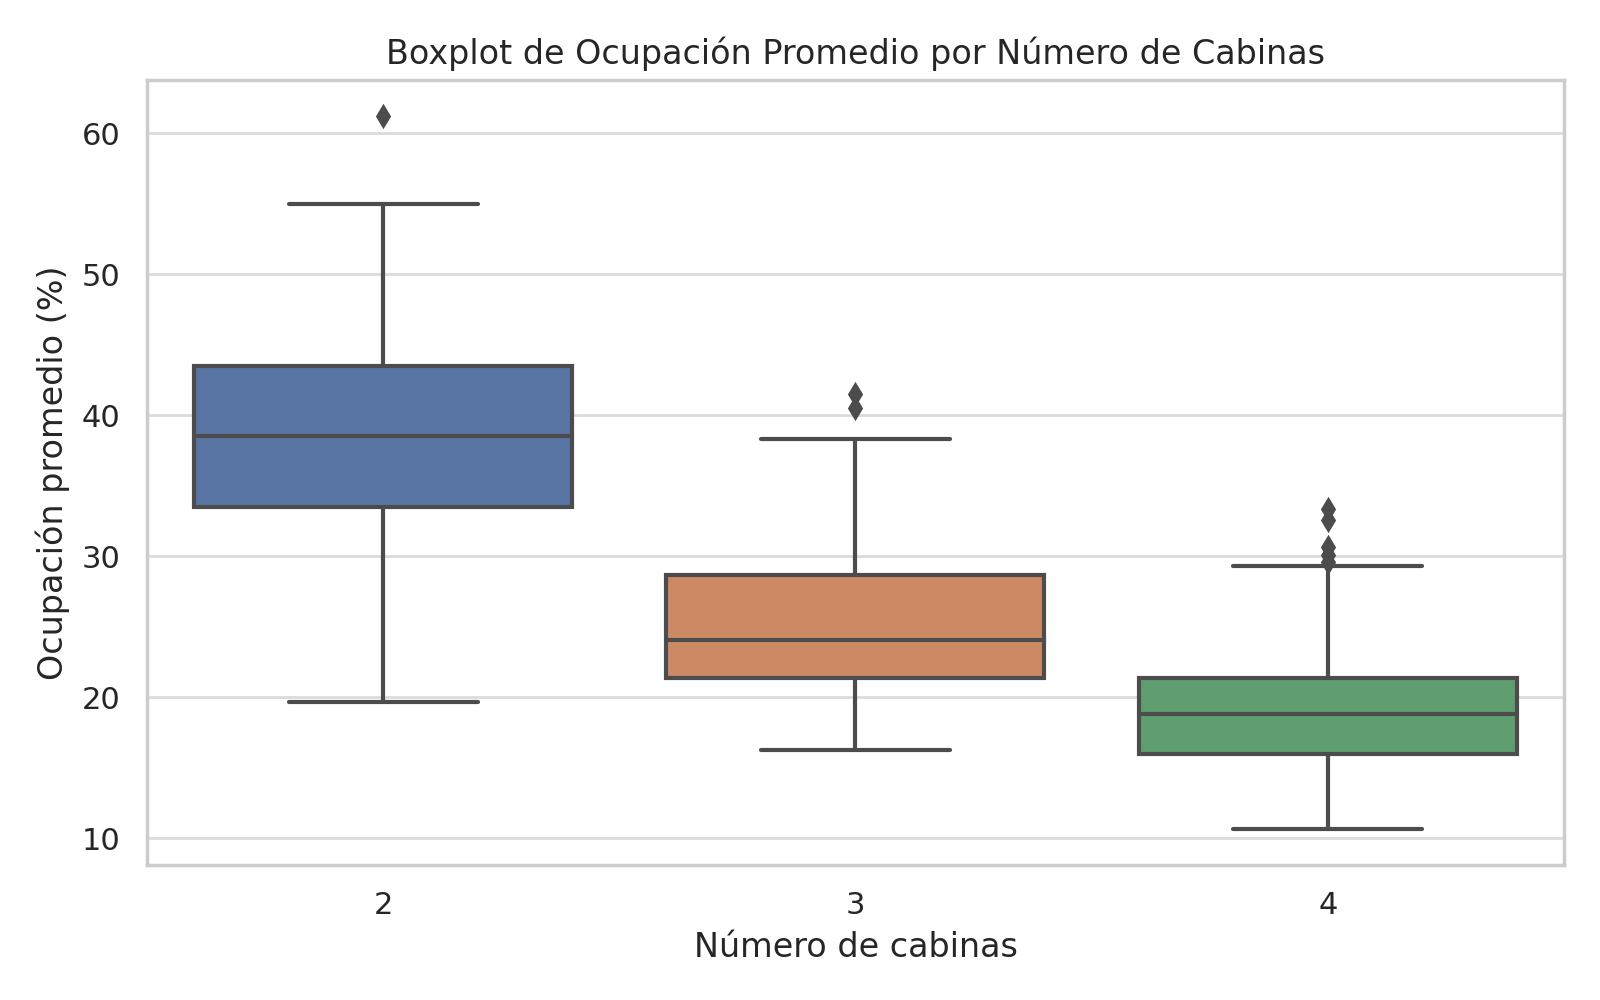
\includegraphics[width=0.8\textwidth]{box_ocupacion.png}
\caption{Boxplot de la ocupación promedio de las cabinas en función del número total.}
\small A medida que aumenta el número de cabinas, la ocupación promedio por cabina disminuye notablemente. Con 2 cabinas, la carga es alta y variable; con 3 o 4, la carga se distribuye mejor y es más estable, lo cual mejora la experiencia del usuario.
\end{figure}

\begin{figure}[H]c
\centering\vspace{-0.5em}
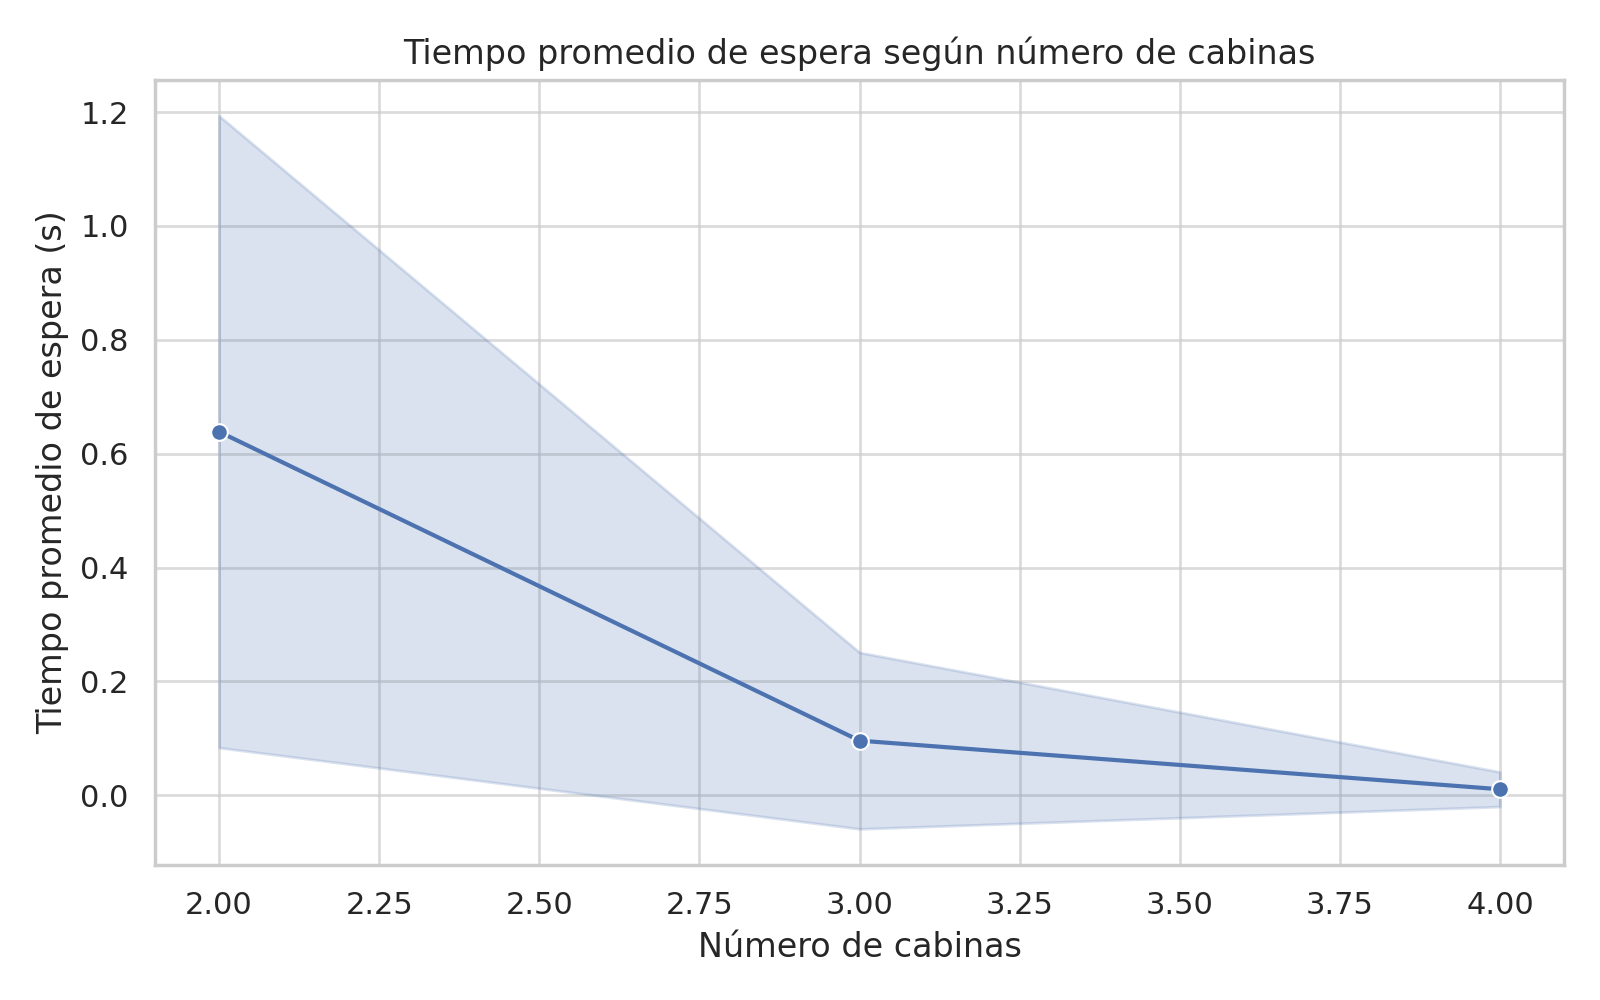
\includegraphics[width=0.8\textwidth]{line_espera.png}
\caption{Tiempo promedio de espera según el número de cabinas.}
\small Existe una relación inversa entre el número de cabinas y el tiempo de espera. El mayor beneficio se obtiene al pasar de 2 a 3 cabinas; a partir de ahí, los beneficios adicionales son menores, indicando rendimientos decrecientes.
\end{figure}

\begin{figure}[H]
\centering\vspace{2.0em}
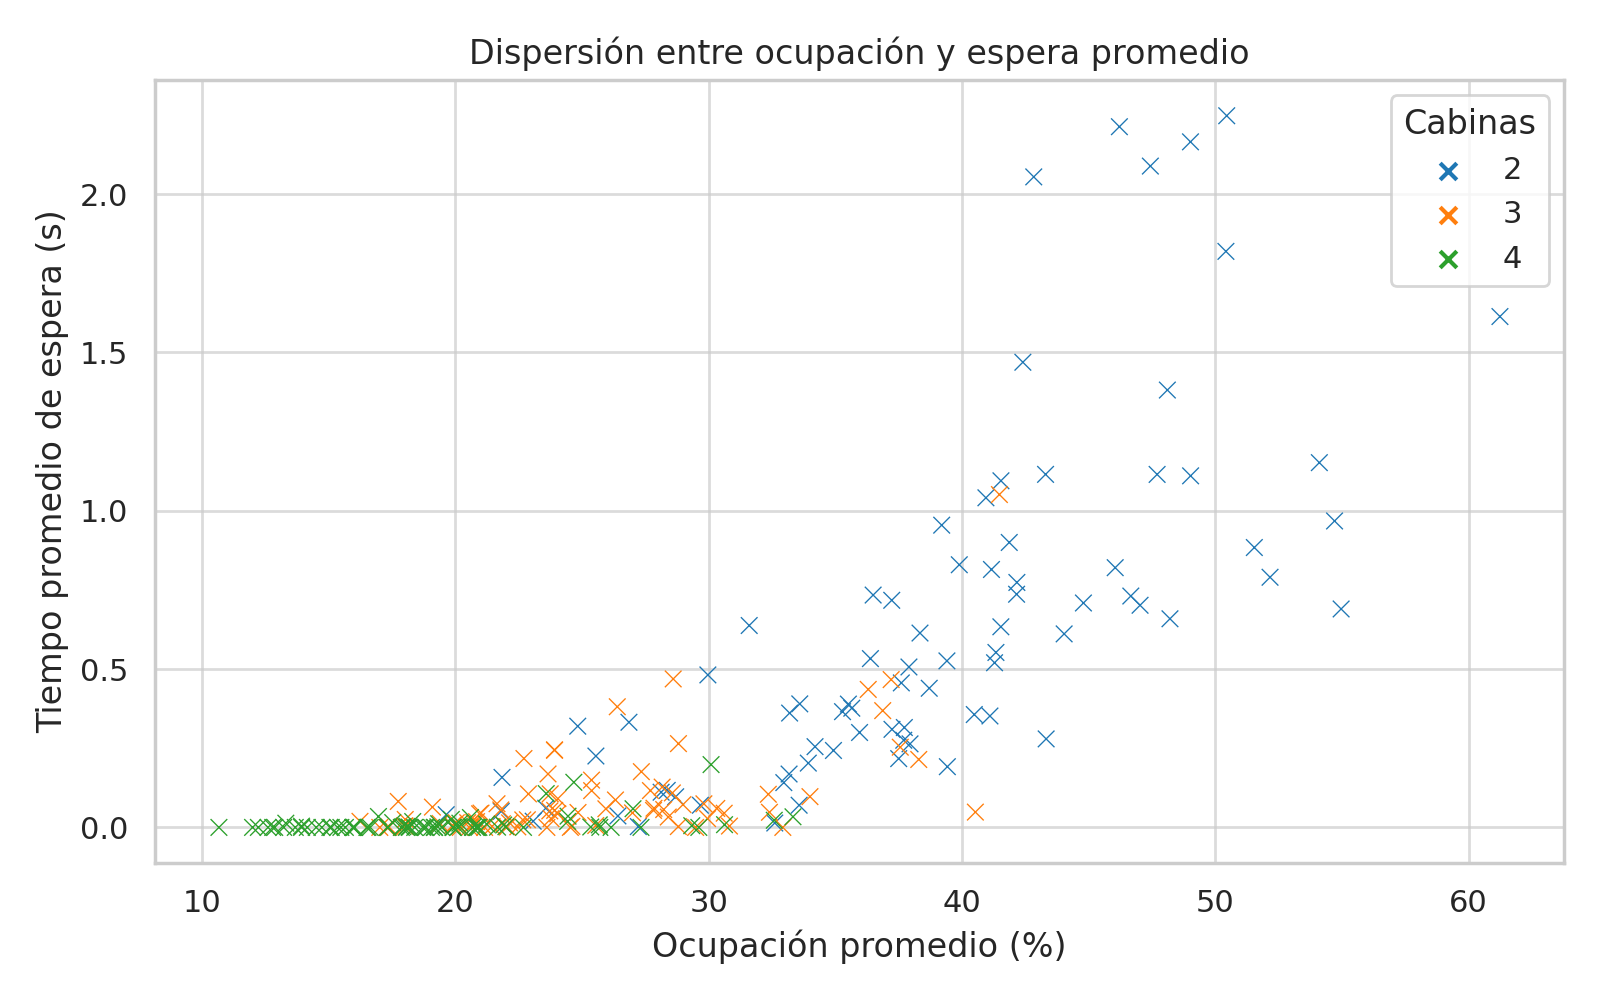
\includegraphics[width=1.0\textwidth]{scatter_ocupacion.png}
\caption{Relación entre ocupación promedio y tiempo de espera.}
\small Se observa una fuerte correlación positiva: cuando la ocupación es alta, también lo es el tiempo de espera. Las simulaciones con más cabinas tienden a situarse en la zona inferior izquierda (baja ocupación y baja espera), lo que indica un mejor desempeño del sistema.

\end{figure}

\newpage

\subsection*{Tabla de Resultados}
A continuación se muestra una muestra de los resultados obtenidos (30 primeras filas):

\begin{table}[H]
    \small
    \setlength{\tabcolsep}{3pt} % reduce espacio entre columnas
    \renewcommand{\arraystretch}{1.2} % ajusta altura de filas
    \begin{tabularx}{\textwidth}{|c|c|c|c|c|c|c|}
    \toprule
    Cabinas & T Total & Tasa Llegada & Tasa Servicio & T. espera & Autos atendidos & Ocupación (\%) \\
    \midrule
    2 & 300 & 0.25 & 0.33 & 0.55 & 75 & 41.34 \\
    2 & 300 & 0.25 & 0.33 & 0.81 & 78 & 41.16 \\
    2 & 300 & 0.25 & 0.33 & 1.11 & 83 & 49.03 \\
    2 & 300 & 0.25 & 0.33 & 0.39 & 73 & 33.60 \\
    2 & 300 & 0.25 & 0.33 & 0.30 & 75 & 35.96 \\
    2 & 300 & 0.25 & 0.33 & 0.35 & 77 & 41.11 \\
    2 & 300 & 0.25 & 0.33 & 0.39 & 75 & 35.52 \\
    2 & 300 & 0.25 & 0.33 & 0.63 & 82 & 41.54 \\
    2 & 300 & 0.25 & 0.33 & 0.14 & 72 & 32.97 \\
    2 & 300 & 0.25 & 0.33 & 0.73 & 74 & 36.49 \\
    2 & 300 & 0.25 & 0.25 & 2.05 & 60 & 42.83 \\
    2 & 300 & 0.25 & 0.25 & 0.71 & 66 & 44.80 \\
    2 & 300 & 0.25 & 0.25 & 0.95 & 74 & 39.20 \\
    2 & 300 & 0.25 & 0.25 & 2.25 & 78 & 50.45 \\
    2 & 300 & 0.25 & 0.25 & 0.97 & 93 & 54.71 \\
    2 & 300 & 0.25 & 0.25 & 0.77 & 67 & 42.17 \\
    2 & 300 & 0.25 & 0.25 & 1.61 & 80 & 61.24 \\
    2 & 300 & 0.25 & 0.25 & 1.15 & 79 & 54.11 \\
    2 & 300 & 0.25 & 0.25 & 0.66 & 69 & 48.21 \\
    2 & 300 & 0.25 & 0.25 & 1.38 & 69 & 48.11 \\
    2 & 300 & 0.20 & 0.33 & 1.04 & 74 & 40.95 \\
    2 & 300 & 0.20 & 0.33 & 0.00 & 55 & 27.22 \\
    2 & 300 & 0.20 & 0.33 & 0.12 & 58 & 28.37 \\
    2 & 300 & 0.20 & 0.33 & 0.26 & 72 & 37.95 \\
    2 & 300 & 0.20 & 0.33 & 0.07 & 53 & 29.67 \\
    2 & 300 & 0.20 & 0.33 & 0.01 & 73 & 32.61 \\
    2 & 300 & 0.20 & 0.33 & 0.05 & 55 & 21.81 \\
    2 & 300 & 0.20 & 0.33 & 0.02 & 50 & 23.07 \\
    2 & 300 & 0.20 & 0.33 & 0.10 & 65 & 28.70 \\
    2 & 300 & 0.20 & 0.33 & 0.32 & 60 & 24.83 \\
    \bottomrule
    \end{tabularx}
    
    \end{table}
    

    \newpage

    \section{Modelo Matemático}

    \subsection{Descripción del modelo como modelos probabilísticos}
    
    El sistema de peaje se modela como una línea de espera \( M/M/c \) :
    \subsection*{Descripción del Modelo $M/M/c$}

El modelo $M/M/c$ es un tipo de modelo de colas ampliamente utilizado para describir sistemas con múltiples servidores que atienden a clientes que llegan de forma aleatoria. Es especialmente útil en contextos donde se desea analizar la eficiencia de los recursos de atención frente a la demanda fluctuante.

\subsubsection*{Características del modelo $M/M/c$}
\begin{itemize}
    \item Las llegadas de clientes siguen un proceso de Poisson (distribución exponencial de tiempos entre llegadas).
    \item Los tiempos de servicio son independientes y distribuidos exponencialmente.
    \item El sistema cuenta con $c$ servidores idénticos que atienden en paralelo.
    \item El estado del sistema depende únicamente del número de clientes presentes en cada instante (propiedad de Markov).
\end{itemize}

\subsubsection*{Usos del modelo $M/M/c$}
\begin{itemize}
    \item Se aplica en áreas como negocios, industria, ingeniería y telecomunicaciones.
    \item Permite estimar la capacidad óptima del sistema para equilibrar costos operativos y calidad del servicio.
    \item Modela situaciones donde los clientes deben esperar en cola antes de ser atendidos.
\end{itemize}

\subsubsection*{Interpretación de la notación $M/M/c$}
\begin{itemize}
    \item \textbf{M} (Markovian): llegadas con distribución de Poisson.
    \item \textbf{M} (Markovian): tiempos de servicio con distribución exponencial.
    \item \textbf{c}: número de servidores paralelos en el sistema.
\end{itemize}

\subsubsection{Aplicación del modelo descrito en el problema }
    
    \begin{itemize}
        \item \( M \): Las llegadas de vehículos siguen un proceso de Poisson con tasa \( \lambda \), indicando que los tiempos entre llegadas son independientes y exponencialmente distribuidos.
        \item \( M \): Los tiempos de servicio en cada cabina son independientes y siguen una distribución exponencial con tasa \( \mu \).
        \item \( c \): Existen \( c \) cabinas de peaje operando en paralelo, actuando como servidores idénticos.
    \end{itemize}
    
    Bajo este modelo, las métricas de interés se calculan mediante las siguientes fórmulas:
    
    \begin{itemize}
        \item **Factor de utilización por servidor**: \( \rho = \frac{\lambda}{c \cdot \mu} \)
        \item **Número promedio de vehículos en el sistema**: \( L = \frac{\lambda W}{c} \)
        \item **Tiempo promedio de espera en la cola**: \( W_q = \frac{L_q}{\lambda} \)
    \end{itemize}
    
    \subsection{Supuestos y restricciones}
    
    Para la validez del modelo \( M/M/c \), se asumen las siguientes condiciones:
    
    \begin{itemize}
        \item **Llegadas y servicios independientes**: Los tiempos entre llegadas y los tiempos de servicio son independientes entre sí.
        \item **Distribuciones exponenciales**: Los tiempos entre llegadas y los tiempos de servicio siguen distribuciones exponenciales.
        \item **Disciplina de servicio FIFO**: Los vehículos son atendidos en el orden de llegada.
        \item **Capacidad infinita de la cola**: No hay límite en el número de vehículos que pueden esperar en la cola.
        \item **Estado estacionario**: El sistema alcanza un equilibrio donde las métricas de rendimiento se estabilizan.
    \end{itemize}
    
    Es importante destacar que, en la práctica, algunas de estas suposiciones pueden no cumplirse estrictamente, lo que podría afectar la precisión del modelo.
    
    \subsection{Comparación de los resultados obtenidos con los resultados experimentales}
    
    Los resultados obtenidos mediante la simulación se compararon con las métricas teóricas del modelo \( M/M/c \). Se observó que:
    
    \begin{itemize}
        \item **Consistencia en tiempos de espera**: Los tiempos promedio de espera obtenidos en la simulación están alineados con los valores teóricos, validando la precisión del modelo en condiciones controladas.
        \item **Variabilidad en la ocupación de las cabinas**: Aunque el modelo teórico asume una ocupación promedio constante, la simulación mostró fluctuaciones debido a la naturaleza estocástica del sistema.
        \item **Impacto del número de cabinas**: Tanto en el modelo teórico como en la simulación, se confirmó que aumentar el número de cabinas reduce el tiempo de espera y la probabilidad de formación de colas largas.
    \end{itemize}
    
    Estas comparaciones indican que el modelo \( M/M/c \) es adecuado para representar el sistema de peaje bajo los supuestos establecidos, aunque es esencial considerar las limitaciones y posibles desviaciones en escenarios reales.
    
La tasa de utilización del sistema se estima como $\rho = \frac{\lambda}{c \cdot \mu}$. Las simulaciones confirman que un aumento en el número de cabinas disminuye el tiempo de espera y la ocupación individual, validando el modelo teórico.

\section{Conclusiones}
La simulación permitió visualizar claramente cómo influyen los parámetros del sistema en su rendimiento. Se comprobó que un mayor número de cabinas reduce significativamente el tiempo promedio de espera. Además, se observó una relación directa entre la tasa de llegada y el nivel de congestión del sistema. Esta herramienta resulta útil para la toma de decisiones en la planificación de infraestructuras viales.



\section*{Bibliografía y enlaces relacionados}

\begin{itemize}
  \item Ross, S. M. (2012). \textit{Simulation}, 5th Edition. Academic Press.
  \item Banks, J., Carson, J. S., Nelson, B. L., \& Nicol, D. M. (2010). \textit{Discrete-Event System Simulation}, 5th Edition. Pearson.
  \item \url{https://en.wikipedia.org/wiki/M/M/c_queue}
  

\end{itemize}

\end{document}
